\subsection{Modello E-R}
Per la realizzazione del modello entità-relazione si è deciso di seguire una strategia mista, isolando l'attività della base di dati in 3 parti principali. 
\begin{itemize}
    \item La prima parte verterà sull'entità Cliente: la creazione di un ordine.
    
    \item La seconda parte si concentrerà sull'entità Prodotto: l'appartenenza ad una specifica categoria e la sua variazione di prezzo in caso di sconto.
    
    \item La terza parte tratterà l'entità Dipendente: la risoluzione di una segnalazione.
\end{itemize}In seguito sarà possibile unire le tre parti utilizzando nuove relazioni tra entità implicate. Ci si pone come obbiettivo la realizzazione di un modello privo di ridondanze e già normalizzato. 

\subsubsection{Cliente}
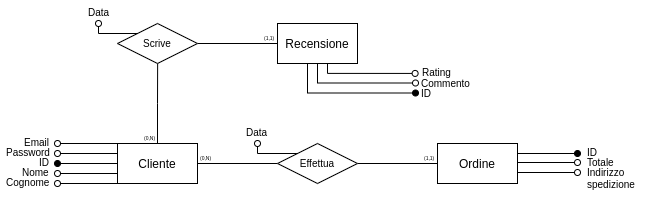
\includegraphics[scale=0.65]{images/cliente.png}
\textbf{Si è scelto di identificare l'entità Cliente attraverso un ID numerico} invece che con\textbf{ l'attributo email}, anche se questo \textbf{rimane altresì una chiave candidata}, \textit{per la quale vige vincolo di univocità}; in questo modo si favorisce la pseudonimizzazione dei dati.

\subsubsection{Prodotto}
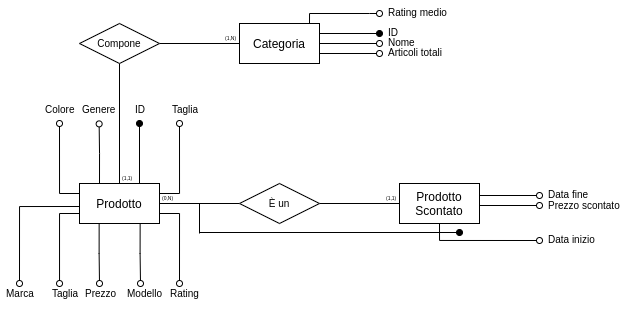
\includegraphics[scale=0.65]{images/prodotto.png}
\textbf{Le chiavi candidate nell'entità prodotto sono ID e la tupla di attributi (Modello, Marca, Taglia, Colore, Genere)}, si è scelto di utilizzare la prima come chiave primaria e rendere univoco l'insieme formato dall'altra.
\subsubsection{Dipendente}
\begin{center}
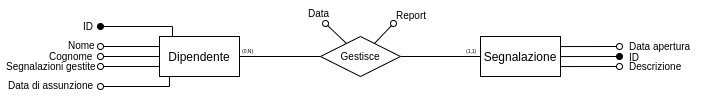
\includegraphics[scale=0.60]{images/segnalazione.png}
\end{center}
\textbf{Viene individuata come chiave primaria dell'entità dipendente l'attributo ID}. La relazione \textit{Gestisce} contiene gli attributi \textit{Data} e \textit{Report} che indicano rispettivamente la data di chiusura della segnalazione e il modo in cui è stata risolta
\subsubsection{Schema finale}
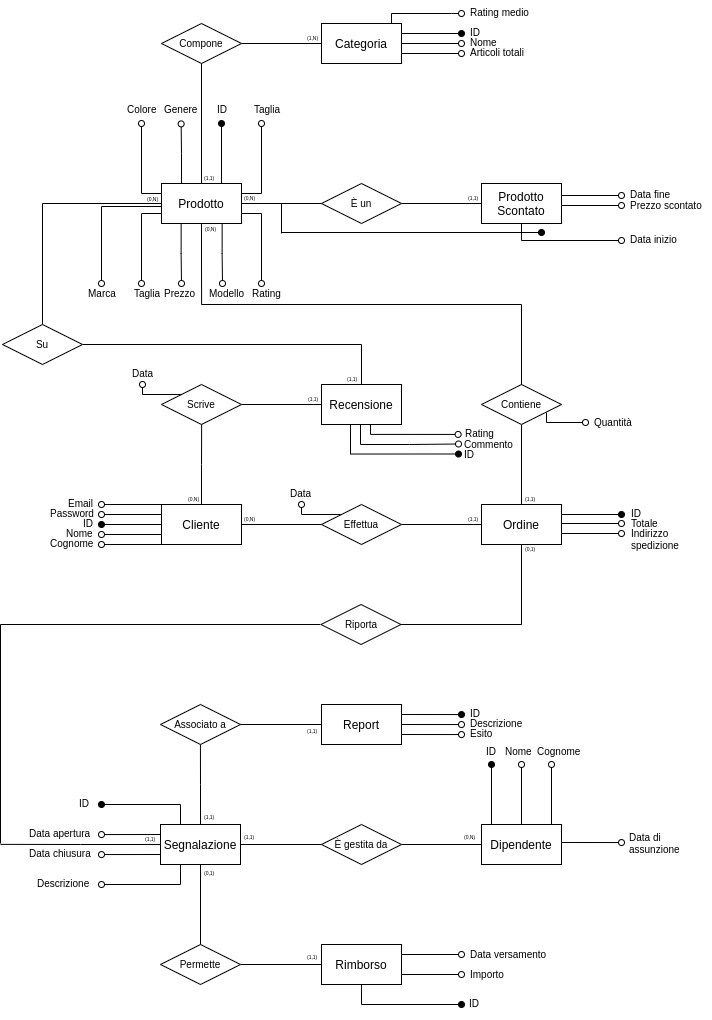
\includegraphics[scale=0.55]{images/schema_finale.png}
\textbf{Lo schema finale è ottenuto unendo gli schemi Cliente, Prodotto e Dipendente}. Si noti che sono state aggiunte le seguenti relazioni: \textit{Recensisce}, \textit{Rimborsa}, \textit{Contiene} e \textit{Riporta}, che fungono da collante tra concetti diversi. \textbf{Dato che la relazione tra Ordine e Segnalazione è 1 a 1 è stato rimosso l'attributo ID da Segnalazione e utilizzato l'ID\_ordine fornito dalla chiave esterna come chiave primaria}.